\documentclass[tikz,border=8pt]{standalone}
\usepackage{amsmath,bm}
\usepackage{avant}
\usetikzlibrary{arrows.meta,calc}
\definecolor{vred}{HTML}{C8260C}
\definecolor{torg}{HTML}{F2961F}
\definecolor{surf}{HTML}{EBEBEB}
\begin{document}
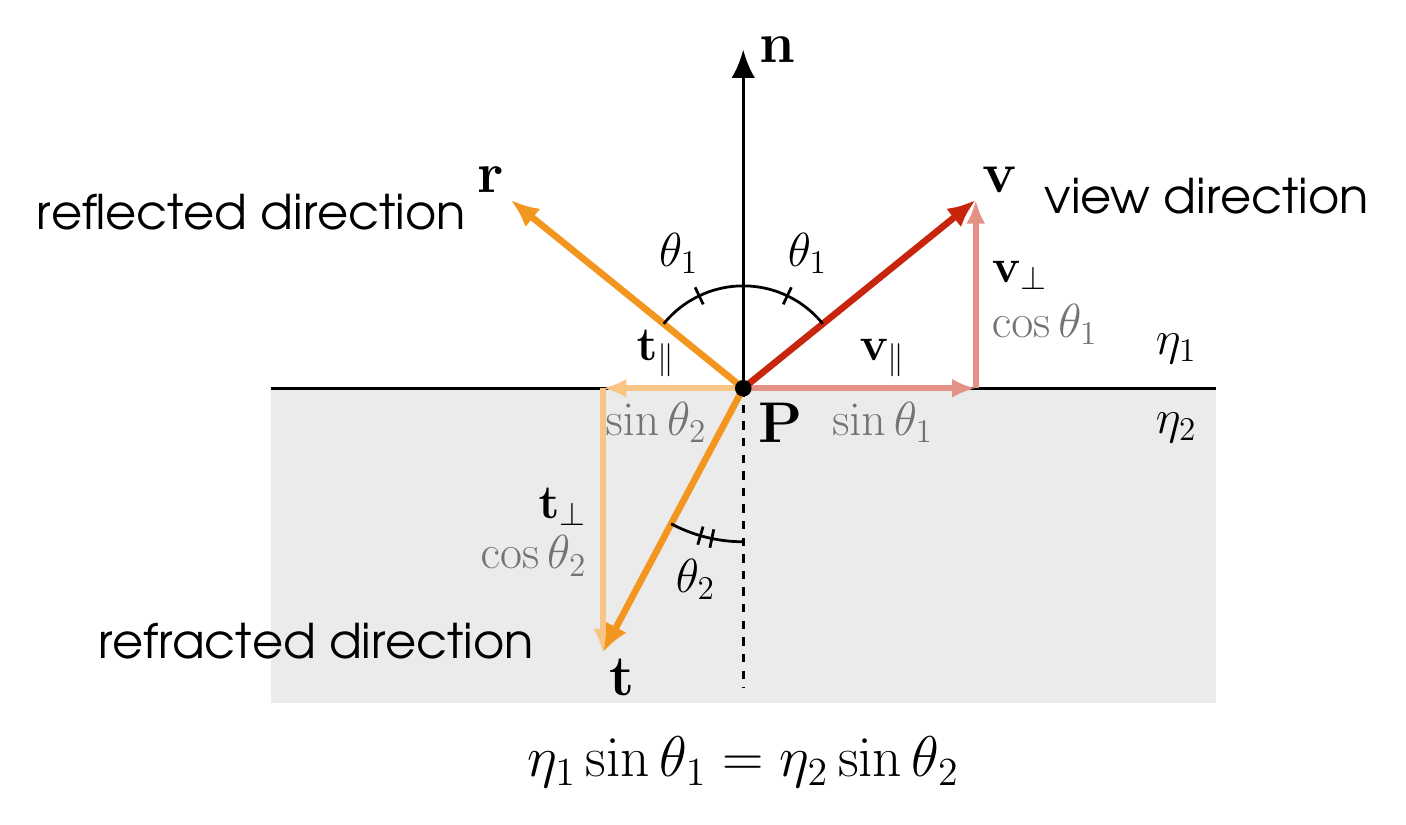
\begin{tikzpicture}[
  font=\LARGE,
  tip/.style={-{Latex[length=3.6mm,width=3mm]}},
  ctip/.style={-{Latex[length=3mm,width=2.4mm]}},
  word/.style={font=\sffamily\LARGE, text=black},
  big/.style={font=\huge, text=black},
  len/.style={font=\LARGE, text=black!55}
]
\def\L{3.8}
\def\ta{51} \def\tb{28}
\coordinate (P) at (0,0);
\coordinate (V) at ({\L*sin(\ta)},{\L*cos(\ta)});
\coordinate (R) at ({-\L*sin(\ta)},{\L*cos(\ta)});
\coordinate (T) at ({-\L*sin(\tb)},{-\L*cos(\tb)});
\coordinate (Vp) at ({\L*sin(\ta)},0);
\coordinate (Tp) at ({-\L*sin(\tb)},0);

% media
\fill[surf] (-6,0) rectangle (6,-4.0);
\draw[line width=1.1pt] (-6,0) -- (6,0);
\node at (5.5,0.5) {$\eta_1$};
\node at (5.5,-0.5) {$\eta_2$};

% normal
\draw[line width=1.2pt, tip] (P) -- (0,4.3) node[big, right=2pt] {$\mathbf{n}$};
\draw[line width=1.1pt, dashed] (P) -- (0,-3.8);

% v components (tip to tail)
\draw[vred!50, line width=2pt, ctip] (P) -- (Vp);
\draw[vred!50, line width=2pt, ctip] (Vp) -- (V);
\node[above] at ($(P)!0.6!(Vp)+(0,0.02)$) {$\mathbf{v}_\parallel$};
\node[len, below] at ($(P)!0.6!(Vp)+(0,-0.05)$) {$\sin\theta_1$};
\node[right] at ($(Vp)!0.6!(V)+(0.08,0)$) {$\mathbf{v}_\perp$};
\node[len, right] at ($(Vp)!0.6!(V)+(0.08,-0.62)$) {$\cos\theta_1$};

% t components (tip to tail)
\draw[torg!55, line width=2pt, ctip] (P) -- (Tp);
\draw[torg!55, line width=2pt, ctip] (Tp) -- (T);
\node[above] at ($(P)!0.62!(Tp)+(0,0.02)$) {$\mathbf{t}_\parallel$};
\node[len, below] at ($(P)!0.62!(Tp)+(0,-0.05)$) {$\sin\theta_2$};
\node[left] at ($(Tp)!0.45!(T)+(-0.08,0)$) {$\mathbf{t}_\perp$};
\node[len, left] at ($(Tp)!0.45!(T)+(-0.08,-0.62)$) {$\cos\theta_2$};

% main vectors
\draw[torg, line width=2.4pt, tip] (P) -- (R) node[big, above left=-2pt] {$\mathbf{r}$};
\draw[vred, line width=2.4pt, tip] (P) -- (V) node[big, above right=-2pt] {$\mathbf{v}$};
\draw[torg, line width=2.4pt, tip] (P) -- (T) node[big, below right=-2pt] {$\mathbf{t}$};
\node[word, anchor=east] at ($(R)+(-0.45,-0.15)$) {reflected direction};
\node[word, anchor=west] at ($(V)+(0.75,0.05)$) {view direction};
\node[word, anchor=east] at ($(T)+(-0.75,0.15)$) {refracted direction};

% angles
\draw[line width=1pt] ({90-\ta}:1.3) arc ({90-\ta}:{90+\ta}:1.3);
\draw[line width=1pt] ({90-\ta/2}:1.18) -- ({90-\ta/2}:1.42);
\draw[line width=1pt] ({90+\ta/2}:1.18) -- ({90+\ta/2}:1.42);
\node at ({90-\ta/2}:1.9) {$\theta_1$};
\node at ({90+\ta/2}:1.9) {$\theta_1$};
\draw[line width=1pt] (-90:1.95) arc (-90:{-90-\tb}:1.95);
\draw[line width=1pt] ({-90-\tb/2-2.2}:1.83) -- ({-90-\tb/2-2.2}:2.07);
\draw[line width=1pt] ({-90-\tb/2+2.2}:1.83) -- ({-90-\tb/2+2.2}:2.07);
\node at ({-90-\tb/2}:2.5) {$\theta_2$};

\fill (P) circle (3pt);
\node[big, below right=2pt] at (P) {$\mathbf{P}$};

\node[font=\huge] at (0,-4.75) {$\eta_1\sin\theta_1 = \eta_2\sin\theta_2$};
\end{tikzpicture}
\end{document}
